\documentclass{article}

\usepackage[paper=letterpaper, margin=1in]{geometry}

\usepackage{tikz}
\usetikzlibrary{shapes,arrows,fit}

\usepackage{siunitx}

\title{Progress Report: Week 1}
\author{LASER Mapping Team}
\date{25 October 2013}

\begin{document}
\maketitle

\section{Project Block Diagram}

The project naturally splits along the hardware-software divide.  There are
further natural subdivisions on both the hardware and software components
(Figure \ref{fig:project-block-diagram}).  The hardware is split into three
components --- the analog laser modulation / phase measurement circuit, the
Inertial Measurement Unit (IMU) and its support circuitry, and the
microcontroller that aggregates the information and transmits it to the PC.  The
software can be structured as a pipeline:
\begin{enumerate}
\item decode the ranging and position integration information coming from the
  hardware,
\item transform the measurements from the hardware's egocentric frame to a
  common world frame,
\item visualize the measurements in the common world frame, and
\item (possibly) lift a representation of the scanned object from the common
  world frame.
\end{enumerate}

\begin{figure}
  \centering
  
% Needs shapes, arrows, and fit libraries.

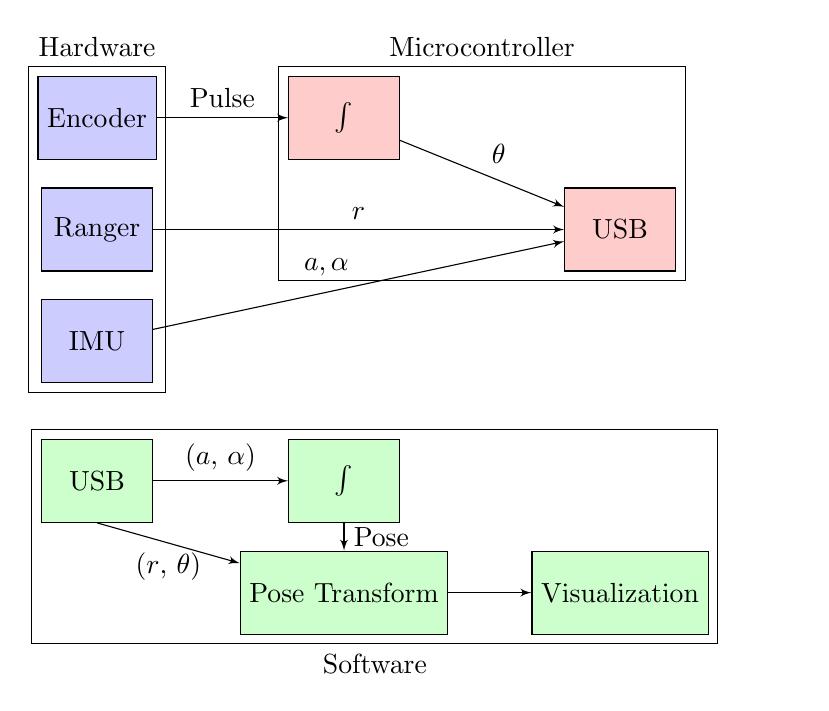
\begin{tikzpicture}[auto, node distance=3cm, >=latex']

% sensor style
\tikzstyle{sn} = [
    draw,
    fill=blue!20,
    rectangle,
    minimum height=3em,
    minimum width=4em
]

% microcontroller style
\tikzstyle{uc} = [
    draw,
    fill = red!20,
    rectangle,
    minimum height=3em,
    minimum width=4em
];

% PC Style
\tikzstyle{pc} = [
    draw,
    fill = green!20,
    rectangle,
    minimum height = 3em,
    minimum width = 4em
]

% Place the nodes.
\matrix [row sep = 1em, column sep = 3em]
{
    \node [sn] (encoder) {Encoder};
    & \node [uc] (enc-int) {$\int$};
    &                         
    \\
    
    \node [sn] (ranger) {Ranger};
    &
    & \node [uc] (usb) {USB};
    & 
    \\
    
    \node [sn] (imu) {IMU};
    &
    &
    \\

    &&&\\

    \node [pc] (pc-usb) {USB};
    & \node [pc] (imu-int) {$\int$};
    &                         
    \\

    % Nothing in first cell.
    & \node [pc] (pose) {Pose Transform};
    & \node [pc] (viz) {Visualization};
    &
    \\ 
};

% Connect the nodes.
\draw [->] (encoder) -- node {Pulse} (enc-int);
\draw [->] (ranger) -- node {$r$} (usb);
\draw [->] (imu) -- node {$a, \alpha$} (usb);
\draw [->] (enc-int) -- node {$\theta$} (usb);
\draw [->] (imu-int) -- node {Pose} (pose);
%\draw [->] (tuple) -- node {To PC} (exit);

\draw [->] (pc-usb) -- node {($a$, $\alpha$)} (imu-int);
\draw [->] (pc-usb.south) -- node [below] {($r$, $\theta$)} (pose);
\draw [->] (pose) -- (viz);

% Draw fitting boxes.
\node[draw, fit= (encoder) (ranger) (imu), label=above:{Hardware}] {};
\node[draw, fit= (enc-int)  (usb), label=above:{Microcontroller}] {};
\node[draw, fit= (pose) (viz) (imu-int) (pc-usb), label=below:{Software}] {};

\end{tikzpicture}

  \caption{Block representation of project dataflow.  Sensed data originates on
    the indicated \textcolor{blue}{hardware components}.  The data is processed
    and assembled into tuples on the \textcolor{red}{microcontroller}, and
    transmitted over the USB connection.  On the attached computer, the
    \textcolor{green}{software pipeline} performs pose normalization, model
    lifting, and visualization.}
  \label{fig:project-block-diagram}
\end{figure}

\section{Member Assignments}

\begin{itemize}
\item Hardware
  \begin{itemize}
  \item Laser Modulation / Phase Measurement: Jeff Terrel, John Boyd, Doug
    Maunder
  \item IMU: Ashton Jackson, Sam Carey
  \item Microprocessor: Clayton Crawford, Sam Carey, Taahir Ahmed
  \end{itemize}
\item Software
  \begin{itemize}
  \item Pose Transform: Clayton Crawford
  \item Visualization: Tengyan Wang
  \end{itemize}
\end{itemize}

\section{Four-Week Timeline}

\begin{enumerate}
\item \emph{1 November 2013:} All hardware schematics finished.  PCB layouts
  finished.  First PCB revision produced.  Software pose transformation and
  simple visualization working on test fixture data.
\item \emph{8 November 2013:} Hardware subunits debugged, second board revision
  laid out and in production.  Tentative microcontroller control of the board.
  Pose transformation and visualization working on test data produced on the
  microcontroller.  Progress on model lifting.
\item \emph{15 November 2013:} Full microcontroller control of the board, data
  passing through the full pipeline.  Planar scanning assembly produced and
  integrated.  Model lifting working.
\item \emph{22 November 2013:} Schedule slack.
\end{enumerate}

\section{Component Statuses}

\subsection{Ranger}
All components have been selected and ordered.  The laser diode will be driven
directly by a programmable oscillator (frequency controlled by
I\textsuperscript{2}C from the microcontroller).  The original signal and the
phototransistor return will be fed into the phase comparator, which outputs
analog representations of the detected phase difference and attenuation.  These
analog signals will be sampled by the dedicated analog to digital converter pins
on the microcontroller.

Schematic capture of the ranger unit has begun and is on-track.

\subsection{IMU}
Both a self-contained chip and a stand-in module (Razor IMU, from SparkFun) have
been identified.  Pads will be placed on the board revision a for both units.
The dedicated chip is accessed via I\textsuperscript{2}C, while the Razor IMU is
accessed via UART.

\subsection{Microcontroller}
The AT90USB1286 from Atmel has been selected as the on-board microcontroller.
Its relevant features are:
\begin{itemize}
\item dedicated I\textsuperscript{2}C and USART (Universal
Synchronous and Asynchronous Receiver and Transmitter) controllers,
\item dedicated USB stack (allowing direct implementation of a USB-to-Serial
  converter, as well as more apropos USB communication standards),
\item 8 dedicated analog to digital converters, as well as a selection of analog
  comparators,
\item on-chip USB bootloader, enabling simple programming over a direct USB
  connection,
\item 16 external interrupts, to allow interfacing with pulse devices such as
  encoders.
\end{itemize}
The Atmel requires some on-board support circuitry, but an open reference design
has been located and schematic capture has begun.

\subsection{Pose Transformation}
The math has been worked out, and implementation is under way.

\subsection{Visualization}
A simple visualization program for visualizing the returned point cloud has been
created.

\end{document}